\documentclass{standalone}

\usepackage{tikz}
\usetikzlibrary{shapes, arrows}
\usetikzlibrary{arrows,calc,decorations.markings,math,arrows.meta}
\usetikzlibrary{positioning}
\usepackage{stackengine}
\usepackage{scalerel}
\usepackage{graphicx}
\usepackage{adjustbox}
\usepackage{calc}

\pgfdeclarelayer{background1}
\pgfdeclarelayer{background2}
\pgfsetlayers{background2,background1,main}

\newcommand\dangersign[1][2ex]{%
  \renewcommand\stacktype{L}%
  \scaleto{\stackon[1.3pt]{\color{red}$\triangle$}{\tiny !}}{#1}%
}


\begin{document}
\trimbox{-0.3cm -0.3cm -0.3cm -0.3cm}{ 
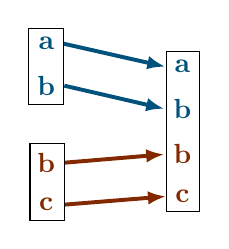
\begin{tikzpicture}

	\definecolor{odmlcolor}{rgb}{0.00,0.32,0.49}
	\definecolor{compcolor}{rgb}{0.51,0.16,0.00}
% 		    \definecolor{color1}{rgb}{}
	\node(a1) [line width = 0pt,align=center,font=\bfseries, text=odmlcolor]{a};
	\node(b1)[below=0.1cm of a1,line width = 0pt,align=center,font=\bfseries, text=odmlcolor]{b};
	
	\node(b2) [below=0.5cm of b1,line width = 0pt,align=center,font=\bfseries, text=compcolor]{b};
	\node(c2)[below=0.1cm of b2,line width = 0pt,align=center,font=\bfseries, text=compcolor]{c};
	
	
	\node(b12) [right=1.5cm of $(b1)!0.3!(b2)$,line width = 0pt,align=center,font=\bfseries, text=odmlcolor]{b};
	\node(b22)[below=0.1cm of b12,line width = 0pt,align=center,font=\bfseries, text=compcolor]{b};
	\node(a)[above=0.1cm of b12,line width = 0pt,align=center,font=\bfseries, text=odmlcolor]{a};
	\node(c)[below=0.1cm of b22,line width = 0pt,align=center,font=\bfseries, text=compcolor]{c};
	
	\coordinate (intersection) at ([shift={(0.75,0)}] $(b1)!0.5!(b2)$);

	
	\begin{pgfonlayer}{background1}
		\draw [draw,fill=white] (a1.north east) rectangle (b1.south west);
		\draw [draw,fill=white] (b2.north east) rectangle (c2.south west);
		\draw [draw,fill=white] (a.north east) rectangle (c.south west);
	\end{pgfonlayer}
	
	\begin{pgfonlayer}{background2}
		\draw[-{Latex[scale=0.7]},line width=0.5mm,odmlcolor] (a1.east) -- (a.west);
		\draw[-{Latex[scale=0.7]},line width=0.5mm,odmlcolor] (b1.east) -- (b12.west);
		\draw[-{Latex[scale=0.7]},line width=0.5mm,compcolor] (b2.east) -- (b22.west);
		\draw[-{Latex[scale=0.7]},line width=0.5mm,compcolor] (c2.east) -- (c.west);
% 		\draw[-{Bar},line width=0.5mm,odmlcolor] (b1.east) -| ([shift={(0,0.1)}] intersection);
% 		\draw[line width=0.5mm,compcolor] (b2.east) -| (intersection);
% 		\draw[-{Latex[scale=0.7]},line width=0.5mm,compcolor] (b2.east) -| (intersection) -- (b12.west);
	\end{pgfonlayer}

\end{tikzpicture}
}
\end{document}